% =============================================================================
% Closed-loop diagram: decide-on-forecast / pay-on-realized (Phase C.2).
%
% Compiles standalone:
%     pdflatex closed_loop.tex
% and is also \input-able into the acmart paper (the tikzpicture is emitted
% verbatim when this file is read inside an existing document class).
%
% Integration note (Phase D): \documentclass is defined in the LaTeX format,
% so the \ifdefined\documentclass guard cannot distinguish standalone vs.
% input mode. The paper defines the sentinel \paperstandaloneinputsentinel
% before \input; when it is defined (input mode) the standalone preamble is
% skipped. Standalone mode is detected by the sentinel being undefined.
% =============================================================================
\ifdefined\paperstandaloneinputsentinel
\else
\documentclass[border=3mm]{standalone}
\usepackage{tikz}
\usetikzlibrary{arrows.meta, positioning}
\begin{document}
\fi
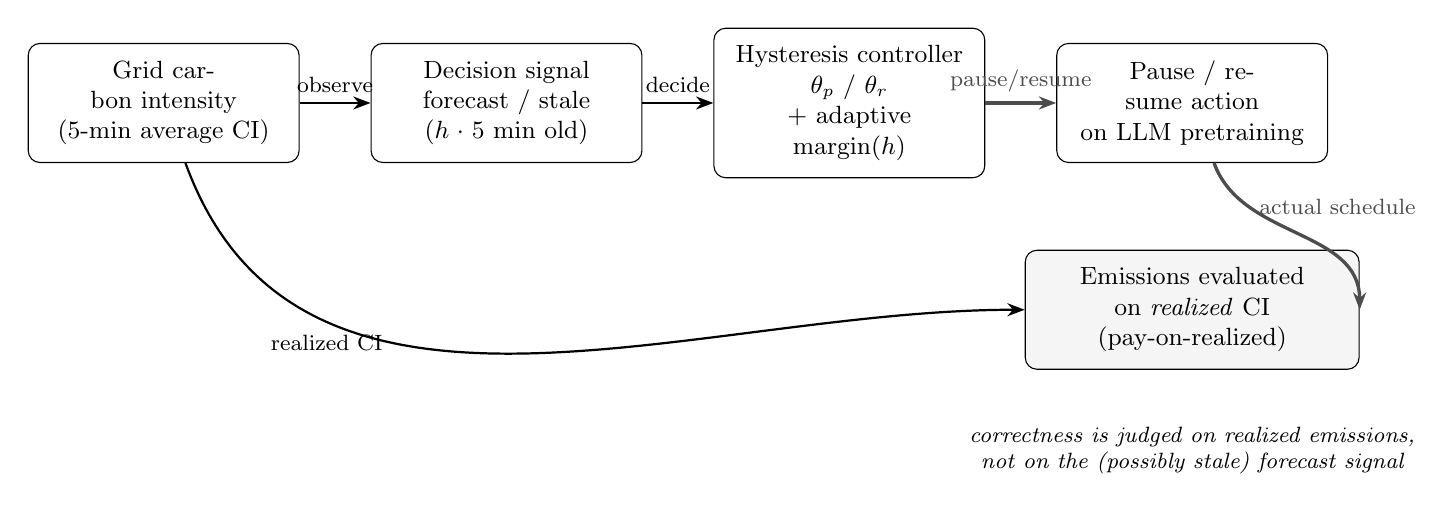
\begin{tikzpicture}[
    node distance=9mm,
    box/.style={draw, rounded corners=1.5mm, align=center, inner sep=2.2mm,
                text width=30mm, font=\small},
    evbox/.style={draw, rounded corners=1.5mm, align=center, inner sep=2.2mm,
                  text width=38mm, font=\small, fill=black!4},
    flow/.style={-{Stealth[length=2.2mm]}, thick},
    actflow/.style={-{Stealth[length=2.2mm]}, very thick, color=black!70},
  ]

  % --- main decision chain (decide on forecast) ---
  \node[box] (ci) at (0,0) {Grid carbon intensity\\ (5-min average CI)};
  \node[box, right=of ci] (sig) {Decision signal\\ forecast / stale\\ ($h \cdot 5$ min old)};
  \node[box, right=of sig] (hyst) {Hysteresis controller\\ $\theta_p$ / $\theta_r$\\ + adaptive margin($h$)};
  \node[box, right=of hyst] (train) {Pause / resume action\\ on LLM pretraining};

  \draw[flow] (ci) -- node[above, font=\footnotesize] {observe} (sig);
  \draw[flow] (sig) -- node[above, font=\footnotesize] {decide} (hyst);
  \draw[actflow] (hyst) -- node[above, font=\footnotesize] {pause/resume} (train);

  % --- pay-on-realized evaluation path ---
  \node[evbox, below=11mm of train] (eval) {Emissions evaluated\\ on \emph{realized} CI\\ (pay-on-realized)};

  \draw[flow] (ci) to[out=-70, in=180] node[left, font=\footnotesize, pos=0.35]
      {realized CI} (eval.west);
  \draw[actflow] (train) to[out=-70, in=90] node[right, font=\footnotesize, pos=0.25]
      {actual schedule} (eval.east);

  % --- annotation of the correctness loop ---
  \node[align=center, font=\footnotesize\itshape, below=6mm of eval]
    {correctness is judged on realized emissions,\\ not on the (possibly stale) forecast signal};
\end{tikzpicture}
\ifdefined\paperstandaloneinputsentinel
\else
\end{document}
\fi
